\section{Исследование и построение решения задачи}
\label{sec:Chapter3} \index{Chapter3}

Для того, чтобы внедрить наше решение в существующий проект по разработке компилятора MyTS,
сначала необходимо тщательно изучить его внутреннее устройство.
Составим обзор компонент компилятора для понимания, как сделать наше решение качественной и логичной частью всего проекта.

\subsection{Исследование компонент компилятора}

\subsubsection{Лексический анализ}

Этот компонент преобразует исходный код в последовательность токенов.
Входные данные должны быть корректной строкой UTF8.
Токены могут быть литералами, знаками препинания или ключевыми словами.
Поскольку в JavaScript существуют контекстуальные ключевые слова, например, \(``\)static\("\) - это ключевое слово внутри тела
класса, но в других местах оно просто идентификатор, токены содержат дополнительное поле keywordType,
которое всегда соответствует соответствующему ключевому слову, независимо от реального типа токена.
Поскольку на этом уровне могут возникать синтаксические ошибки, лексический анализатор может
генерировать соответствующие ошибки.

\subsubsection{Область видимости}

Структуры областей видимости - это сущности, в которых хранятся переменные.
Каждая область видимости имеет родителя - область по вложенности выше, все объявления классов, переменных и функций,
которые хранятся в специальной таблице переменных.
Эта таблица содержит строку в качестве ключа и структуру переменной в качестве значения.

\subsubsection{Объявления}

Объявления типа \hl{var a} или \hl{let b} во время синтаксического анализа преобразуются в структуры объявлений, которые
как раз добавляются в специальную таблицу, описанную выше.
Каждое объявление знает имя и узел AST дерева, к которому оно относится.

\subsubsection{Переменные}

Структура переменной содержит в себе структуру объявления, к которой она привязана, область видимости, в которой она
находится, а также фактический статический тип переменной и различные вспомогательные флаги.
Переменные не создаются по умолчанию.
Объявления преобразуются в переменные, если они проходят проверку в рамках области видимости.
Тип переменной неизвестен во время синтаксического анализа и заполняется позже анализатором типов.

\subsubsection{Привязка переменных}

В компиляторе существует специальный компонент, который создает и проверяет все привязки объявлений к области видимости.
Эти привязки, как было сказано ранее, хранятся в таблице переменных.
Сам по себе этот этап не является отдельным анализом.
Каждая проверка привязки запускается в процессе синтаксического анализа.
В настоящее время триггерами могут быть:

\begin{itemize}[left=2em]
    \item Создание новой области видимости.
    \item Добавление объявления в текущую область видимости.
    Если в результате проверки добавить привязку не получается, возникает синтаксическая ошибка.
\end{itemize}

\subsubsection{Синтаксический анализ}

Синтаксический анализ осуществляет специальный компонент компилятора, который называется Парсер.
Этот анализ логично происходит после лексического разбора исходного кода программы.
Парсер является одним из основных компонент и работает параллельно с этапом привязки переменных.
Синтаксический анализ является однопоточным, и входные данные обрабатываются только один раз.
Для парсинга выбран синтаксический анализатор LR(1), поэтому он видит только следующий токен,
но может заглянуть в следующую точку кода.
Однако из-за новых возможностей стандарта ES2015 список параметров лямбда функций и шаблоны деструктурирования
больше не могут быть корректно прочитаны, заглядывая только на один токен вперед.
В этих сценариях синтаксический анализатор работает в отказоустойчивом режиме, что означает,
что он следует менее строгой грамматике, чем стандартная.
Всякий раз, когда закрывающий токен для этих языковых элементов найден или не найден, выполняется обход построенного AST
дерева и проверка его правильности в соответствии с правилами грамматики.
По мере того как AST строится во время синтаксического анализа, также создается дерево областей видимости.
Как только парсер обрабатывает очередной блок кода или функцию, запускается этап привязки переменных,
который создает для них новую область видимости и привязывает их к ней.
Поскольку время жизни этих областей совпадает со временем жизни соответствующих узлов AST дерева,
структуры представляющие узел также сохраняют у себя эти области видимости.
Всякий раз, когда считано объявление переменной, выполняется проверка привязки.
Таким образом, в общем случае синтаксический анализатор уведомляет инструмент проверки привязок только о том,
что он обнаружил новое начало области видимости или объявление новой переменной.

\subsubsection{AST дерево}

ASTNode - это базовый класс всех узлов, сгенерированных парсером.
Узел AST хранит в себе данные о позиции в исходном коде, родительский узел и другие атрибуты,
которые добавляются дочерним классам при наследовании.

\subsubsection{Анализ имен переменных}

После того, как исходный код обработан парсером, AST проходит анализ имен переменных.
После него создается класс программы, содержащий AST дерево, позиции переменных в исходном коде и некоторые метаданные.
Главной целью этого анализа является определение типа переменной для обеспечения эффективной многопоточной компиляции
без блокировки, не считая планирования потоков.
Переменная может быть локальная или лексическая.
Во время обхода AST дерева мы ссылаемся на уже сгенерированные области видимости, присвоенные statement узлам,
чтобы определить, в какой области мы на самом деле находимся.
Всякий раз, когда мы оказываемся в узле, представляющий собой имя (идентификатор) переменной,
анализатор пытается разрешить ее тип из текущей области.
Если у переменной нет конфликтов с какой-либо другой переменной из области видимости
(чаще всего это область видимости функций или цикла), переменная объявляется как локальная.
В противном случае она получает лексический индекс из ближайшей области видимости и помечается как лексическая.
Каждый раз, когда из области видимости запрашивается лексический слот на переменную, область становится лексической.
Это означает, что во время компиляции в начале функции должно быть создано так называемое лексическое окружение.
В этом анализе мы также определяем, является ли локальная переменная внутри объявления цикла частью замыкания
внутри его тела.
Результат этого анализа определяет, должны ли цикл или его объявление быть лексическими или нет.
Таким образом, перед переходом непосредственно на стадию кодогенерации AST обрабатывается только один раз.
Каждая область видимости содержит в себе информацию о том, нуждается ли она в лексическом окружении или нет,
и каждая переменная знает, является ли она лексической или нет.

\subsubsection{Анализатор типов}

Этот компонент семантически анализирует код, используя AST дерево, области видимости и переменные.
Анализатор обходит AST дерево и проверяет каждый узел, используя определенную виртуальную функцию,
перегруженную для всех узлов по-своему.
Когда анализатор обнаруживает узел с объявлением какой-либо переменной, он выполняет ее поиск во всех областях видимости
по степени их вложенности друг в друга.
Как только найдено объявление этой переменной в какой-то области видимости, анализатор присваивает тип выражения к узлу
дерева, если он задан явно, либо использует для этого вывод типов.

\begin{itemize}[left=2em]
    \item При незаданной аннотации, тип объявленной переменной выводится с помощью ее определения (выражения-инициализатора).
    \item При объявлении функции анализатор создает для нее сигнатуру, которая состоит из параметров в заданном порядке
    и типа возвращаемого значения.
    Этот тип в свою очередь выводится из явно указанной аннотации или типа выражения, следующего за return в теле функции.
    \item При объявлении интерфейса анализатор создает объектный тип, который хранит в себе все поля и их типы, а также
    сигнатуры методов и конструкторов интерфейса.
    С точки зрения анализатора интерфейс и класс практически ничем не различаются (только способом хранения супертипов).
    \item При объявлении псевдонима типа (type alias) анализатор использует тип, который этому псевдониму и присваивается.
\end{itemize}

\subsubsection{Типы сущностей в анализаторе}

Как только тип объявления вычислен, ему присваивается значение ts-типа объявленной переменной.
Используя специальную структуру для хранения этого ts-типа, анализатор может проверять на валидность выражения
присваивания, бинарные или унарные операции, вызовы функций и конструкторов, доступы к полям класса и наследование.
Важно отметить, что statement не создает тип, это делают только выражения.

\begin{itemize}[left=2em]
    \item Statement проверяется только семантически.
    Например, если statement проверяется на наличие у него выражения-условия,
    которое имеет тип void вместо boolean, анализатор сообщает об ошибке, поскольку выражения типа void не могут быть
    проверены на истинность.
    \item Выражения, с другой стороны, по своей сути порождают типы.
    Например, бинарное выражение \hl{5 + 6} порождает числовой тип.
\end{itemize}

Стоит отметить, что виртуальная функция проверки, переопределенная для всех узлов дерева, всегда возвращает
значение nullptr для statement узлов и тип сущности для обычных выражений.

\subsubsection{Виды отношений между типами}

В определенный момент во время семантического анализа анализатор типов должен соотнести различные типы друг с другом.
Например, если переменной присвоено значение a = 15, анализатор сравнивает тип переменной a с типом
инициализатора, который представляет собой числовое литеральное выражение, приводимое к числовому типу.
Если a был объявлен как \hl{let a: string}, то это присвоение приведет к ошибке, поскольку тип string не может быть
присвоен типу number.
В зависимости от операции, производимых с переменными, существует 4 различных типа отношений:

\begin{itemize}[left=2em]
    \item Отношение идентичности: отношение является истинным, если два сравниваемых типа абсолютно идентичны.
    Оно используется при повторном объявлении переменной или поля, и это наиболее сильное отношение.
    \item Отношение подтипирования: отношение является истинным, если один тип сущности анализатора является подтипом
    другого.
    Оно также истинно и для идентичных типов.
    Чаще всего (для обычных несложных объектов) подтипирование выражается простым наследованием.
    \item Отношение присваивания: отношение является истинным, если тип с правой стороны может быть присвоен типу
    с левой стороны.
    Оно используется при обработке присваиваний, операндов бинарных выражений, наследования (отношение базового и дочернего класса),
    а также для проверки совместимости типа возвращаемых выражений из return с типом возвращаемого значения, объявленного в функциях.
    \item Отношение приведения: отношение является истинным, если тип в левой части может быть приведен к типу в правой части.
    Оно используется при работе с операторами сравнения и явными приведениями типов.
    Это самое слабое отношение и оно, вообще говоря, не сильно отличается от отношения присваивания.
\end{itemize}

\subsubsection{Сигнатуры функций}

Сигнатуры создаются для функций и методов, и они могут быть явно объявлены в теле интерфейса или класса,
например, используя следующий синтаксис: \hl{(a: number, b: string): number}.
Существует два типа сигнатур: сигнатуры функций и конструкторов.
Сигнатуры функций используются для проверки корректности вызовов функций.
Например, если объявление функции с именем func1 было объявлено с сигнатурой (a: string, b: string), то оно не может
быть вызвано с меньшим или большим количеством параметров, чем 2, и аргументы вызова функции должны быть присваиваемы
типу параметра сигнатуры в правильном порядке.
Таким образом, анализатор выдаст ошибку в любом из этих случаев:
func1(1), func1(1, 2, 3), func1("foo"), func1(2, "bar").
Сигнатуры конструкторов идентичны по своим правилам.
Разница лишь в том, что они используются при создании объектов и, соответственно, в выражениях с ключевым словом new.

\subsubsection{Понижающие трансформации AST дерева}

Понижающее трансформации AST дерева - это фаза преобразований, работающая, в основном, после анализатора и перед кодогенерацией,
во время которой происходит обход AST дерева и модификация некоторых его узлов с заменой отфильтрованных выражений на
более простые и низкоуровневые конструкции.
Стоит уточнить, что не все понижающие проходы выполняются после анализатора.
На самом деле, некоторые проходы трансформируют AST дерево и до семантического анализа.
У каждого прохода имеются предусловие и постусловие.
Как видно из названий, предусловие является триггером для запуска трансформации дерева для конкретного узла, а
постусловие проверяет, что преобразование было успешным и не нарушило структуру и инварианты AST дерева.
Преимущества внедрения понижающих трансформаций следующие:

\begin{itemize}[left=2em]
    \item Абстрагирование разнообразной логики – трансформации различных частей дерева могут быть написаны независимо
    друг от друга
    \item Упрощение кодогенерации
    \item Легкость отладки.
    Дает возможность распечатать и проанализировать состояние AST дерева до и после какой-то определенной трансформации.
\end{itemize}

Недостатки lowering проходов:

\begin{itemize}[left=2em]
    \item Увеличение времени компиляции
    \item Возможная утеря отладочной информации
    \item Основательный семантический анализ проводится до большинства lowering проходов.
    После трансформаций не исключено, что состояние AST дерева станет некорректным.
    \item Подходит только для некоторых задач
\end{itemize}

Примеры lowering фаз, которые осуществляют трансформацию определенных конструкций языка и AST дерева:

\begin{itemize}[left=2em]
    \item Обработка лямбда-функций, генерация для них объекта.
    \item Раскрытие объектных литералов
    \item Boxing и unboxing переменных
    \item Замена каких-либо выражений на вызовы специальных функций
    \item Оптимизации
\end{itemize}

\subsubsection{Кодогенерация из промежуточного представления}

Кодогенерация осуществляется параллельно для каждого AST узла.
Специальный класс, исполняющий роль этого этапа, контролирует все функции, которые генерируют байт-код или
управляют ресурсами.

\subsubsection{Аллокация регистров}

Формат исполняемого файла требует, чтобы все параметры размещались в конце локальных регистров.
Поскольку в данном языке есть инициализация полей и переменных по умолчанию, а также rest параметры, от локальных
регистров требуется выполнение определенных стандартных действий.
Для этого нам нужно загружать соответствующие параметры в регистры.
Номер соответствующего регистра зависит от количества используемых локальных регистров, что является циклической
зависимостью.
Для разрешения этой проблемы, была представлена следующая структура регистра:

\begin{table}[h]
    \centering
    \begin{tabular}{|c|c|c|c|c|c|}
        \hline
        локальный n & локальный 1 & локальный 0 & параметр 0 & параметр 1 & параметр n \\
        \hline
        ... & 65534 & 65535 & 65536 & 65537 & ... \\
        \hline
    \end{tabular}
\end{table}

Таким образом, во время генерации кода выделяемые регистры располагаются в порядке убывания, и при
необходимости все spill-fill инструкции генерируются сразу в нужном месте.
Как только вся кодогенерация завершена, становится известно количество всех выделенных локальных регистров, а аргументы
генерируемых инструкций преобразуются следующим образом:

\begin{itemize}[left=2em]
    \item Локальные регистры отображаются в диапазоне uint16\_t
    \item Параметры вычисляются как UINT16\_MAX - общее количество регистров.
\end{itemize}

\subsubsection{Выделение регистров для локальных переменных при кодогенерации}

Каждый раз, когда очередной этап кодогенерации доходит до области видимости блока или функции, соответсвующий класс
обрабатывает локальные переменные.
На этом шаге известно, является ли переменная лексической или локальной.
Лексические переменные не затрагиваются, поскольку они уже получили свой лексический индекс во время
анализа имен переменных.
Поскольку индекс регистра, в котором лежит локальная переменная, считывается или записывается только классом кодогенерации,
присваивание регистра на этом этапе безопасно.
Всякий раз, когда область видимости заканчивается, эти регистры освобождаются и могут быть повторно
использованы позже.

\subsubsection{Разрешение имен переменных}

При генерации байткода всякий раз, когда требуется разрешить имя переменной (идентификатор),
используется тот же метод, что и при анализе имен переменных:
начинается поиск имени переменной из текущей области видимости и отслеживается, сколько областей мы проходим.
В зависимости от результатов поиска принимается решение, какой байт-код нам нужно сгенерировать для разрешения:

\begin{itemize}[left=2em]
    \item Местных
    \item Лексических
    \item Модульных
    \item Глобальных
\end{itemize}

переменных.
К этому времени информация о типе переменной, вычисленной анализатором, уже доступна, но в данный момент
не используется.

\subsubsection{Узел промежуточного представления}

Узел промежуточного представления имеет свой определенный класс в структуре компилятора.
Каждая инструкция из архитектуры набора команд (ISA), сгенерированная из специального файла, имеет свою структуру,
которая содержит только необходимые операнды.
Исключением является только самый базовый класс инструкции, который содержит список операндов каждого типа.
Этими типами операндов могут быть:

\begin{itemize}[left=2em]
    \item Виртуальный регистр - VReg
    \item Иммидиат - Imm
    \item Строка - StringView
    \item Метка - Label
\end{itemize}

Кроме того, каждый узел промежуточного представления содержит в себе узел AST дерева,
чтобы получать информацию о позиции какой-либо сущности в исходном коде для генерации отладочной информации.
В конце каждой кодогенерации узлы промежуточного представления будут преобразованы в инструкции другого IR.
Во время преобразования:

\begin{itemize}[left=2em]
    \item Сохраняются строковые операнды, которые позже будут добавлены в таблицу строк сгенерированной программы
    \item Операнды VReg переназначаются на их реальные регистровые индексы.
\end{itemize}

\subsubsection{Преобразование в следующее промежуточное представление}

Этот этап преобразует класс кодогенерации в функциональный класс стороннего промежуточного представления, который уже
потом используется для оптимизации и записи всех сущностей в исполняемый файл.
Список сущностей, которые отдаются в следующее промежуточное представление:

\begin{itemize}[left=2em]
    \item Метки
    \item Try-catch блоки
    \item Инструкции
    \item Отладочная информация
\end{itemize}

Также передаются все общеиспользуемые данные.
Такими данными могут быть, например, строки и литералы.
Всякий раз, когда класс кодогенерирации отдает какие-то данные промежуточного представления этому этапу,
заполняется таблица функций с сущностями из следующего промежуточного представления.

\subsection{Схематичное устройство компилятора}

Кратко проанализировав и описав выше основные компоненты компилятора, которые позволяют трансформировать исходный код на
языке MyTS в некое промежуточное представление с дальнейшей оптимизацией и генерацией байт-кода,
стоит представить обобщенную схему работы данного компилятора:

\begin{figure}[h]
    \centering
    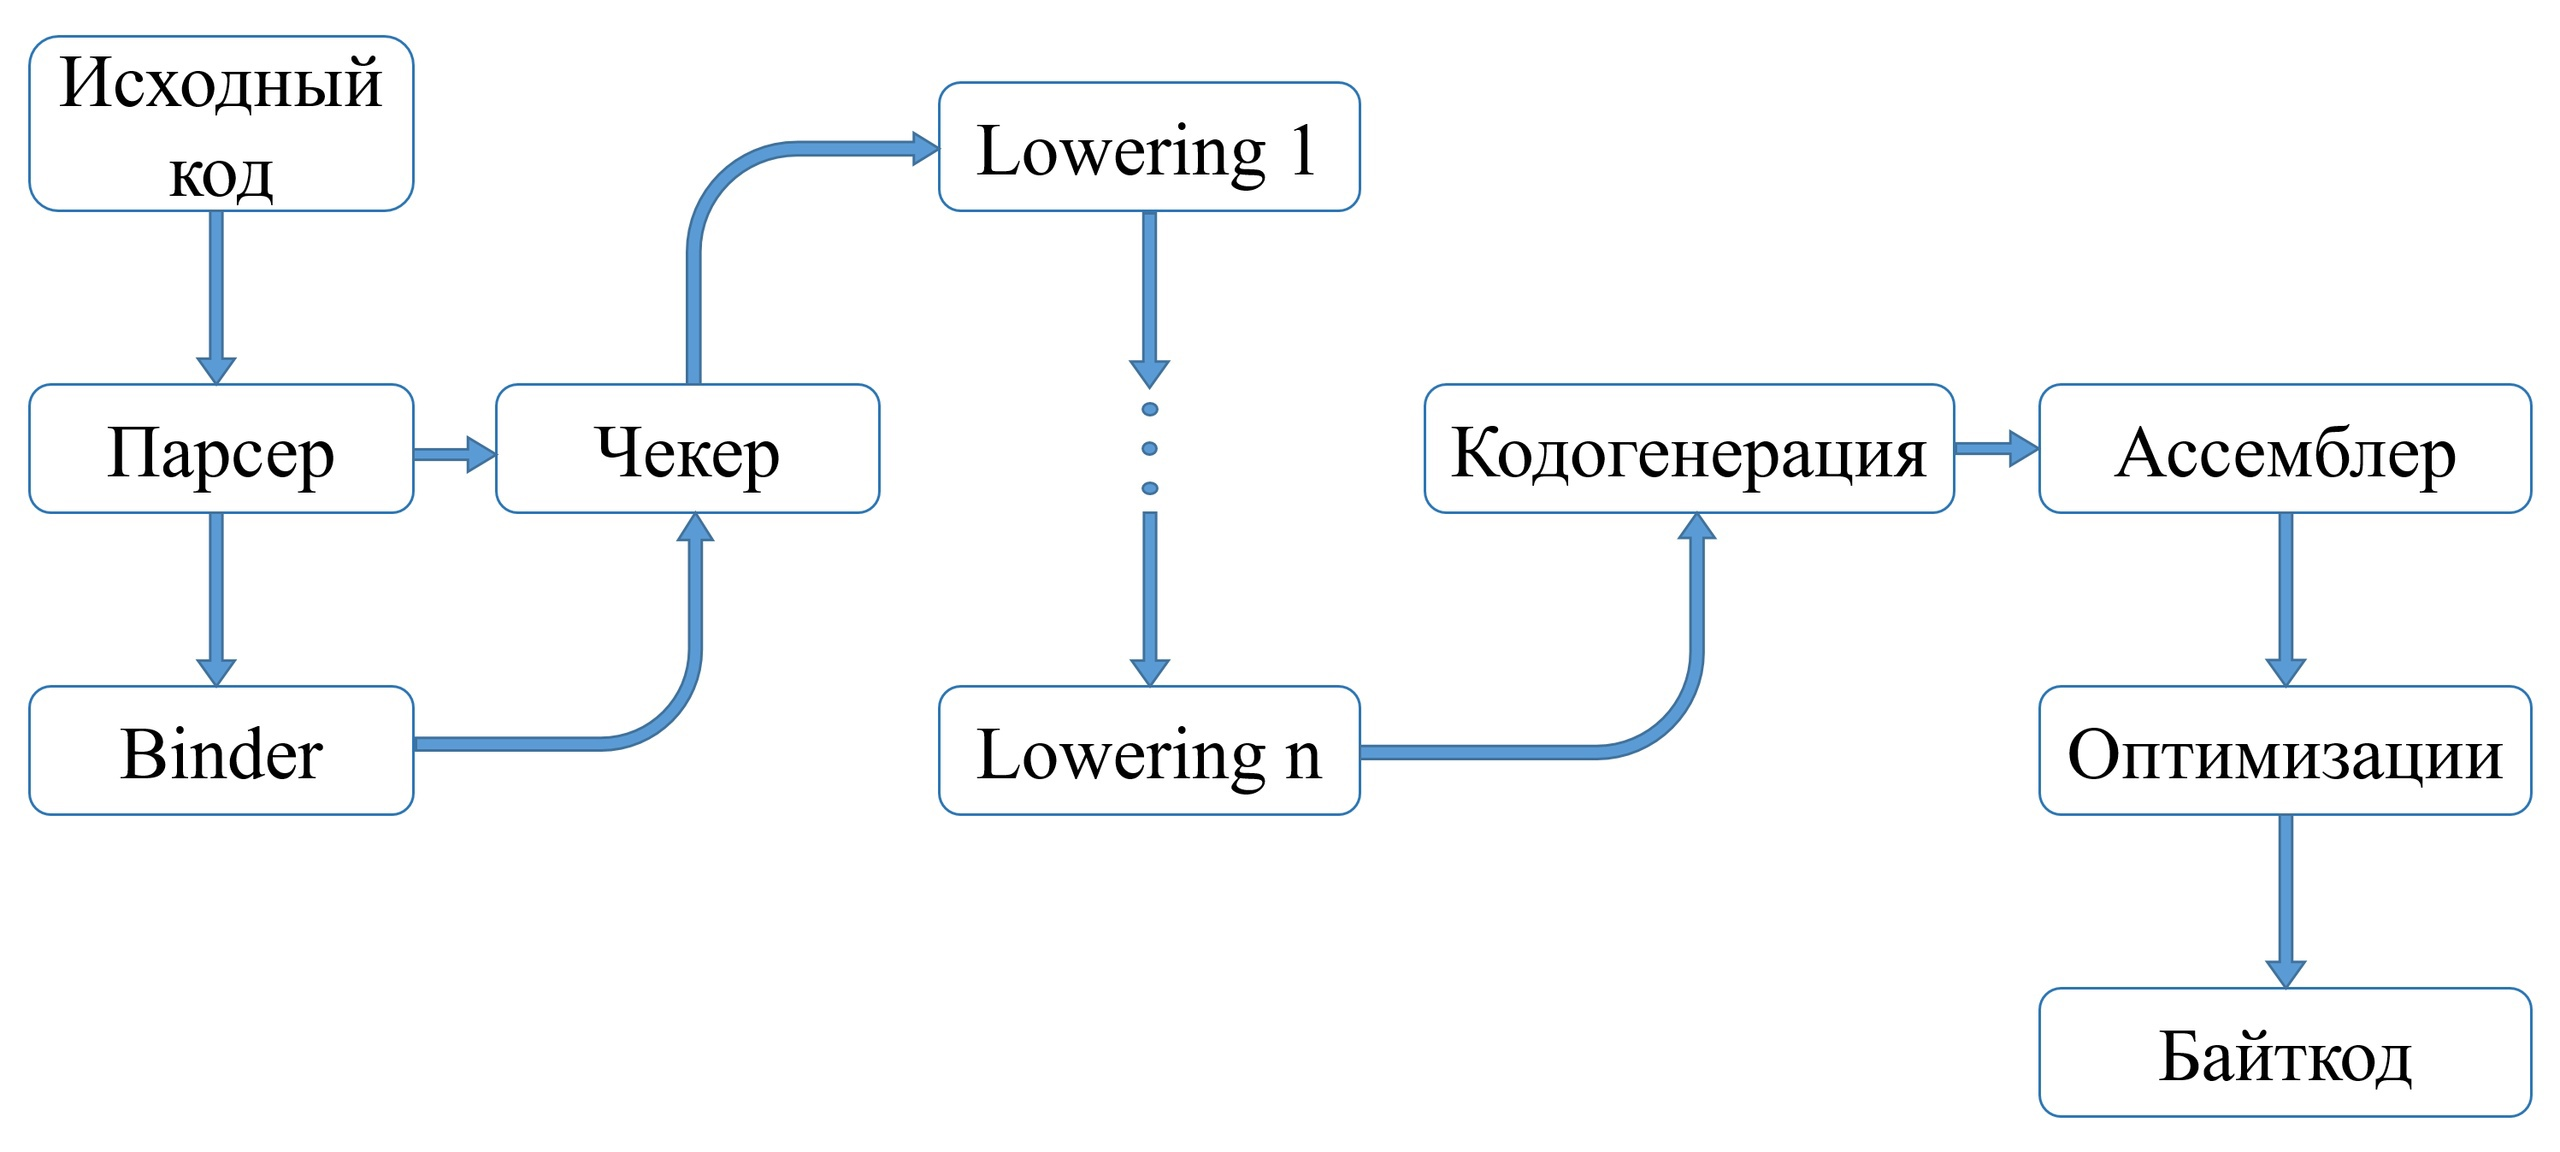
\includegraphics[scale=0.18]{Lowering1.jpg}
    \caption{Схема работы компилятора}\label{fig:figure}
\end{figure}

\subsection{Boxing и unboxing операции}

Boxing и unboxing - это важные концепции в языках программирования, особенно в тех, где есть поддержка
объектно-ориентированного программирования и системы типов.
Эти операции позволяют преобразовывать примитивные типы данных в объекты (boxing) и наоборот (unboxing), что
обеспечивает единообразное обращение к данным и их управление.

\subsubsection{Определения}

Boxing - это процесс преобразования примитивного типа данных в соответствующий ему объект.
Например, целочисленное значение типа int может быть упаковано в объект Integer в языке Java или в объект
System.Int32 в языке C\#.
Этот процесс автоматически осуществляется компилятором или средой выполнения.
Unboxing, наоборот, представляет собой процесс извлечения значения из упакованного объекта и его преобразования
обратно в примитивный тип данных.
Например, извлечение целочисленного значения из объекта Integer в Java или из объекта System.Int32 в C\#.

\subsubsection{Преимущества и Недостатки}

Одним из основных преимуществ использования boxing и unboxing является возможность работы с примитивными типами данных
в контексте объектно-ориентированного программирования.
Это позволяет использовать примитивные типы в качестве аргументов методов, сохранять их в коллекциях и передавать в
качестве параметров в методы, требующие объектов.
Однако, следует помнить, что процесс boxing и unboxing может быть затратным с точки зрения производительности, особенно
при выполнении операций в циклах или при работе с большими объемами данных.
Это связано с тем, что при упаковке и распаковке происходит создание дополнительных объектов и процесс их управления.

\subsubsection{Примеры в разных языках программирования}

Рассмотрим пример использования boxing и unboxing в языке программирования Java:
\begin{lstlisting}[language=Java,label={lst:lstlisting22}]
    int num = 10;
    Integer obj = num;

    Integer obj2 = new Integer(20);
    int num2 = obj2.intValue();
\end{lstlisting}
В первом случае на второй строке происходит автоматический boxing, а во втором на четвертой строке - явный unboxing.

В Kotlin также существует поддержка для boxing и unboxing, но благодаря удобным функциям и умному подходу к типизации,
эти операции редко требуются.
Однако, в некоторых случаях они могут быть полезны.
В Kotlin есть возможность использовать inline-функции и inline-классы, которые могут помочь избежать ненужных boxing и
unboxing.
Компилятор Kotlin может автоматически оптимизировать код, встроив вызовы функций и классов прямо в месте их использования.
Хорошая практика в языке способствует минимизации их использования в пользу примитивных типов и эффективных структур данных.

В TypeScript, поскольку это язык сильной типизации, прямого аналога операций boxing и unboxing, как в Java или C\#, нет.
Однако язык MyTS, используемый в нашей работе, статический и в нем присутствуют такие операции в отличие от TypeScript.
Поэтому при присвоении каких-то примитивных значений типу объединения придется использовать лишние вызовы для упаковки
или распаковки примитивов.
Мы постараемся в данной работе минимизировать такие дорогостоящие операции и оптимизировать байт-код под среду исполнения.

\subsection{Семантика и синтаксис объединений}

Для корректной поддержки семантики и синтаксиса TypeScript согласно поставленной задаче, необходимо изучить примеры
кода, где используются объединения, и спецификацию языка MyTS\@.
Рассмотрим описание объединений в исследуемом нами статически типизированном языке программирования и сравним их
функциональность с объединениями из TypeScript.

\subsubsection{Определение объединений}

Грамматика union типов задается тем же способом, что и в TypeScript, и может быть записана следующим образом:

\begin{lstlisting}
    unionType:
        type|literal ('|' type|literal)*
    ;
\end{lstlisting}
Здесь можно заметить, что компонентами объединения могут быть как обычные типы (пользовательские, встроенные,
примитивные, и т.д), так и литеральные, представляющие собой конкретные значения встроенных типов.
Все составляющие объединения должны быть перечислены через вертикальную черту.
Объединение является ссылочным типом, однако в данной работе мы сделаем определенное исключение для оптимизации кода.

Согласно спецификации, ошибка времени компиляции возникает, если тип в правой части объявления union типа приводит к
циклической ссылке.
Если в объединении используется примитивный тип, то выполняется автоматический boxing, чтобы сохранить
ссылочный характер типа.
Сокращенная форма объединения типов позволяет определить тип, который имеет только одно значение (литерал), например

\begin{lstlisting}
    type UT = 42
\end{lstlisting}

Рассмотрим различные примеры кода на TypeScript, которые будут валидны и в языке MyTS.

\subsubsection{Объединения с пользовательскими классами и доступ к полям}

Дадим определения некоторых пользовательских классов A, B и C:

\begin{lstlisting}
    class A {
        fieldA: number = 41
        field: number = 5
    }
    class B {
        fieldB: number = 42
        field: number = 6
    }
    class C {
        fieldC: number = 43
        field: number = 7
    }
\end{lstlisting}
То есть в каждом классе есть поле с именем field и одинаковым типом number, а также другое поле, уникальное для каждого
класса.
Тогда мы имеем право создать следующие псевдонимы (type alias) на объединения пользовательских классов с примитивным типом
number и без него:

\begin{lstlisting}
    type UT1 = A|B|C|number
    type UT2 = A|B|C
\end{lstlisting}
где UT1 может быть экземпляром класса A, B, C или числом, а UT2 может быть экземпляром класса A, B или C\@.
Далее рассмотрим фрагменты кода, которые используют определенные нами типы объединения.

\begin{lstlisting}
    let u1: UT1 = new A();
\end{lstlisting}
Здесь переменной u1 присваивается тип UT1, и ей присваивается экземпляр класса A\@.
На этом этапе u1 конкретно является типом A\@.
Рассмотрим доступ к свойству field:
\begin{lstlisting}[escapechar=!]
    u1.!\colorbox{lightcoral}{field}!
\end{lstlisting}
TypeScript здесь обязан выдать ошибку, потому что u1 может потенциально быть числом, а число не имеет свойства field.
Чтобы безопасно получить доступ к свойству field, нужно сузить тип переменной:

\begin{lstlisting}
    if (u1 instanceof A) {
        u1.fieldA
        (u1 as A).fieldA
    }
    u1 = 45
\end{lstlisting}
Условие \hl{if (u1 instanceof A)} сужает тип u1 до A внутри блока.
Внутри этого блока \hl{u1.fieldA} и \hl{(u1 as A).fieldA} оба безопасно получают доступ к fieldA\@.
После чего значение 45 типа number присваивается переменной u1, что допустимо, поскольку UT1 включает тип number.
Рассмотрим пример использования u2:

\begin{lstlisting}
    let u2: UT2 = new C()
    u2.field
\end{lstlisting}
Здесь u2 имеет тип UT2, и ей присваивается экземпляр класса C.
Поскольку u2 может быть только A, B или C, доступ к u2.field безопасен, потому что все эти классы имеют свойство field
с одним и тем же типом поля number.

Фрагменты кода выше показывают, как объединённые типы TypeScript, сужение типов с помощью instanceof и приведения типов
(as) работают вместе для обеспечения безопасности типов и гибкости кода.

\subsubsection{Объединения с литералами}

Дадим определения следующих псевдонимов для объединений литеральных типов:

\begin{lstlisting}
    type UT3 = 5
    type UT4 = 5 | 7 | 9
\end{lstlisting}
где UT3 — это литеральный тип, который может принимать только значение 5, а UT4 — это объединение, которое может
принимать только конкретные значения 5, 7 или 9.
Рассмотрим использование типа UT3:

\begin{lstlisting}[escapechar=!]
    let u3: UT3 = 5
    !\colorbox{lightcoral}{u3}! = 4
\end{lstlisting}
Здесь переменной u3, имеющей тип UT3, сначала присваивается значение 5.
Это допустимо, поскольку UT3 может быть только литералом 5.
Однако на следующей строчке TypeScript выдаёт ошибку, потому что u3 может принимать только значение 5, и попытка
присвоить ей 4 недопустима.
Далее рассмотрим использование типа UT4:
\begin{lstlisting}
    let u4: UT4 = 5
    if (u4 == 5) {
        u4 = 7;
    } else if (u4 == 7) {
        u4 = 9;
    }
\end{lstlisting}
Здесь переменной u4 присваивается тип UT4, и ей присваивается значение 5.
Это допустимо, поскольку UT4 может иметь значения литералов 5, 7 или 9.
Далее в условном ветвлении идет проверка значения u4 на равенство какому-либо литералу, после чего оно изменяется в
зависимости от результата проверки.
Если u4 равно 5, то ему присваивается значение 7.
Если u4 равно 7, то ему присваивается значение 9.
В любом случае эти присваивания допустимы, так как 7 и 9 входят в допустимый диапазон значений типа UT4.
Однако, если мы попытаемся сравнить значение u4 с литералом, которого нет в объединении, то согласно спецификации
должна произойти ошибка времени компиляции для такого кода:
\begin{lstlisting}
    u4 == 99
\end{lstlisting}

Эти примеры демонстрируют, как TypeScript использует литеральные и объединённые типы для обеспечения строгой типизации
и контроля значений переменных.

\subsubsection{Нормализация объединений}

Нормализация объединённых типов позволяет минимизировать количество типов и литералов в объединённом типе, сохраняя
при этом безопасность типа.
Некоторые типы или литералы могут быть также заменены на более общие типы.
Формально, объединённый тип $A_1$ | \ldots | $A_n$, где N > 1, может быть сокращён до типа $B_1$ | \ldots | $B_k$, где k <= n,
или даже до не объединённого типа или значения T\@.
В последнем случае T может быть примитивным типом или литералом, изменяющим ссылочную природу типа объединения.

Процесс нормализации предполагает выполнение следующих шагов один за другим:

\begin{itemize}[left=2em]
    \item Линеаризация: Если объединение состоит из двух или более вложенных объединений, они сливаются в одно объединение.
    Например,

    \hl{($A_1$ | $A_2$) | ($A_3$ | $A_4$)} превращается в \hl{$A_1$ | $A_2$ | $A_3$ | $A_4$}.
    \item Удаление идентичных типов: Если в объединении есть несколько одинаковых типов, то они сокращаются до одного.
    Например,

    \hl{string | string} превращается в \hl{string}.

    То же после boxing: Если один тип в объединении может быть преобразован в другой через boxing, то они заменяются на
    более общий тип.
    Например, \hl{number | Number} становится \hl{Number}.
    \item Удаление идентичных значений: Если в объединении есть несколько одинаковых литералов, они сокращаются до одного.

    Например, \hl{5 | 5 | 5} превращается в \hl{5}.
    \item Доминирование Object: Если в объединении есть тип Object, то все остальные не-nullish типы удаляются.

    Например, \hl{777 | Object} становится \hl{Object}.
    \item Если среди объединённых типов присутствует тип never, то он удаляется (\hl{number | never} => \hl{number}).
    \item Если в объединении есть непустая группа числовых типов, то в объединении остаётся только самый крупный числовой тип,
    а остальные удаляются.
    Любой числовой литерал, который подходит под самый крупный числовой тип в объединении, удаляется.
    Другими словами, если в объединении есть числовые типы, то остаётся наибольший из них.
    Например, \hl{int | short | float | 2} становится \hl{float}.
    \item Удаление литералов, принадлежащих типам: Если литерал принадлежит типу, который является частью объединения,
    то он удаляется.
    Например, \hl{5 | number} превращается в \hl{number}.
    \item Удаление литералов, принадлежащих unboxed типам чисел: Если числовой литерал принадлежит unboxed типу одного
    из объединённых числовых типов, он удаляется.
    Например, \hl{Int | 3.14 | Float} превращается в \hl{Int | Float}.
    \item Доминирование базового типа в иерархии классов: Если в объединении есть класс и его производный класс,
    то побеждает базовый класс.
    Например:
        \begin{lstlisting}
            class Base {}
            class Derived1 extends Base {}
            class Derived2 extends Base {}
            Base | Derived1 => Base
            Derived1 | Derived2 => Derived1 | Derived2
        \end{lstlisting}
    \item Этот шаг выполняется рекурсивно до тех пор, пока не останется взаимно совместимых типов или пока объединённый
    тип не сократится до одного типа:
    \begin{itemize}[left=2em]
        \item Если объединённый тип включает два типа $A_i$ и $A_j$ (i != j), и $A_i$ совместим с $A_j$, то в объединённом типе
    остаётся только $A_j$, а $A_i$ удаляется.
        \item Если $A_j$ совместим с $A_i$, то в объединённом типе остаётся $A_i$, а $A_j$ удаляется.
    \end{itemize}
\end{itemize}

Результатом процесса нормализации является либо нормализованный union тип, либо один единственный тип, не являющийся
объединением, причем он может быть и не ссылочным типом.

\subsection{Инструкция для доступа к полю объединения}

Для более эффективной генерации байт-кода, в архитектуре системы команд (ISA), данной нам среде исполнения, предусмотрены
специальные инструкции:

\begin{itemize}[left=2em]
    \item LON\_INST (Load Object field by Name Instruction) - загрузка в аккумулятор поля объекта по имени
    \item SON\_INST (Store something into Object field by Name Instruction) - загрузка значения
    из аккумулятора в поле объекта
\end{itemize}

Для того, чтобы инструкция в среде исполнения отработала корректно, необходимо сгенерировать специальный класс в
байт-коде, который называется \hl{union\_member\_access}.
В этом классе должно быть объявлено поле с тем именем и типом, которое существует для всех компонент объединения.
Позже среда исполнения сможет получить доступ к полю объединения на основе этих данных, несмотря на то
какой конкретно тип объекта хранится в объединении, причем без приведения к более узкому типу.

\newpage
